%(1) Algorithm
%(2) Time series result and validation
%(3) Deformation maps
%(4) Data now available for stakeholders, what people can do (brief discussion on Peter's work, we could use one of his figures I have).
%



\chapter{Robust Time Series Methods for Long-term Nonlinear Deformation}
\label{CHAP:5-robust-ts}


In this chapter, we present a method for robustly extracting slowly-varying surface deformation over long time periods.
% from time series with large noise. 
We perform a temporal smoothing using the robust Locally Weighted Scatterplot Smoothing (LOWESS) technique \citep{Cleveland1979RobustLocallyWeighted} on noisy surface deformation time series derived using SBAS.
%The method extends the ideas behind the outlier-removal technique presented in Chapter \ref{CHAP:4-GRL}.
%Compared to the alternatives presenting in Section \ref{sec:ch4-method-compare}, 
The LOWESS smoothing technique easily accounts for nonlinear deformation while also suppressing the strong summer tropospheric noise.
We demonstrate the technique on both synthetic data and on three paths of Sentinel-1 data over the Permian Basin.
The cumulative results show subtle basin-wide uplift features arising after 4-5 years of heavy sustained wastewater injection.



%- Problem: 
%1. Longer time series, the linear assumption becomes less valid.  This is at odds with the balance of using more measurements to average out tropospheric noise
%2. Methods incorporating temporal smoothness constraints (Find a few. e.g. Karissa? other temp smooth solvers...) or temp lienar filtering methods get influenced by strong tropo days. Even with smoothing, there are anomalous bumps 
%	- can get interpreted as deformation if we assume that all movements remaining after filtering are due to the low-pass deformation
%	

\section{Algorithm}
%	\bm{A \phi} = \bm{\Delta \phi} + \bm{\epsilon} . \label{eq:ch2-sbas-A}
%where  $\bm{A}$ is the system design matrix, and $ \bm{\epsilon}  $ is the vector of interferogram-specific noise sources (e.g. $ \Delta \phi_{decor}, \Delta \phi_{unwrap}, \Delta \phi_{scat}, \Delta \phi_{n} $ from Equation \eqref{eq:ch2-insar-noise-terms}).
Consider a time series of $N$ LOS phase delays for a single pixel,  $ \bm{\phi} = \left[\phi_0, \phi_1, \ldots, \phi_{N-1} \right]^T $ sampled at time intervals $ \bm{t} = \left[t_0, \ldots, t_{N-1} \right]^T $, solved from the SBAS linear system (Equation \eqref{eq:ch2-sbas-A}).
We can write each element $\phi_i$ as a sum of surface deformation and atmospheric delay,
\begin{equation}
	\phi_i = \frac{4 \pi}{\lambda} \left(d_i + \alpha_i \right)
\end{equation}
where $ d_i$ and $\alpha_i$ are the surface deformation and atmospheric delay on the $i$th day, and $ \lambda $ is the radar wavelength.
Here we consider the case that the interferogram-specific noise sources (e.g. $  \Delta \phi_{decor}, \Delta \phi_{unwrap}, \Delta \phi_{scat}  $) have been properly accounted for in the inversion process so that the remaining noise in  $ \bm{\phi} $ is predominantly from the atmospheric delay $ \bm{\alpha} =\left[\alpha_0, \ldots, \alpha_{N-1} \right]^T $.
%Since deformation is usually the quantity of interest,
Our goal is to separate the vector of surface deformation $ \bm{d} =  \left[d_0, d_1, \ldots, d_{N-1} \right]^T $ from the atmospheric noise $ \bm{\alpha} $.
% consists of all terms in Equation \eqref{eq:ch2-insar-noise-terms} which affect the phase of a SAR acquisition and all interferograms containing that acquisition

The most widely used non-parametric methods for separating $ \bm{d} $ from $ \bm{\alpha} $ rely on the fact that the turbulent component of $\bm{\alpha}$ is uncorrelated in time, while most deformation sources show strong temporal correlation.
%There are several approaches to separating $ \bm{d} $ from $ \bm{\alpha} $.
%If a functional model of deformation is known to exist (e.g. linear, transient jumps \citep{Chen20142010SlowSlip, Fielding2017SurfaceDeformationNorth}, seasonal variations \citep{Murray2018ShortLivedPause}, or a combination \citep{Riel2018QuantifyingGroundDeformation}), a model fit can be performed on the noisy $ \bm{\phi} $ time series to extract the model parameters of interest.
%However, when the deformation model is not known, methods usually rely on the fact that the turbulent component of $\bm{\alpha}$ is uncorrelated in time \citep{Emardson2003NeutralAtmosphericDelay} while most deformation sources show strong temporal correlation.
For example, the authors of \cite{Ferretti2000NonlinearSubsidenceRate} and \cite{Berardino2002NewAlgorithmSurface} estimated $\bm{\alpha}$ by performing a high-pass temporal filter on each pixel followed by spatially low pass filtering the residual phase.
The temporal high pass filter was implemented by subtracting a low-pass filtered version of $ \bm{\phi} $ (using a triangular filter in \cite{Ferretti2000NonlinearSubsidenceRate}) from the original unfiltered version.
% (i.e. $ \phi $)
%used spatial and temporal filters on $\bm{\Delta \phi}$.
%These filters are expanded upon and compared in Chapter \ref{CHAP:5-robust-ts}, where a new robust filter is presented to separate deformation from atmospheric noise.
One difficulty with the triangular filter and linear methods enforcing temporal smoothness
% other moving-average filters (e.g. a Gaussian filter) 
is that the filter coefficients are non-adaptive; noisier atmospheric conditions will be weighted the same as calmer conditions \citep{Liu2012SatelliteRadarInterferometry}.
This can cause considerable leakage of noise from severe weather conditions into the deformation estimate of adjacent days (e.g. the regularized solution shown in Figure \ref{fig:ch4-compare-ts}a).

% From Liu, 2012
% Given a good spatial density of coherent targets and a short satellite repeat orbit the filtering method used in the standard PSInSAR (see Ferretti et al. (2000)) provides a simple and fast means to separate APS from temporally correlated deformation signal. However, the separation is usually not optimal and can be erroneous when there are acquisition gaps in the time series or for acquisitions taken under extreme weather conditions such as thunderstorms. This is because the approach weights APS equally for all acquisitions and remove it by a window-based (e.g., triangle, Gaussian) temporal low-pass filter. The filter is not adaptive and its parameters (e.g., temporal correlation length) are up to the users to specify. A good filter, however, should weight APS per acquisition differently according to its significance and be self-adjustable based on the input data to optimize its parameters towards an optimal filtering.


\begin{figure}
	\centering
	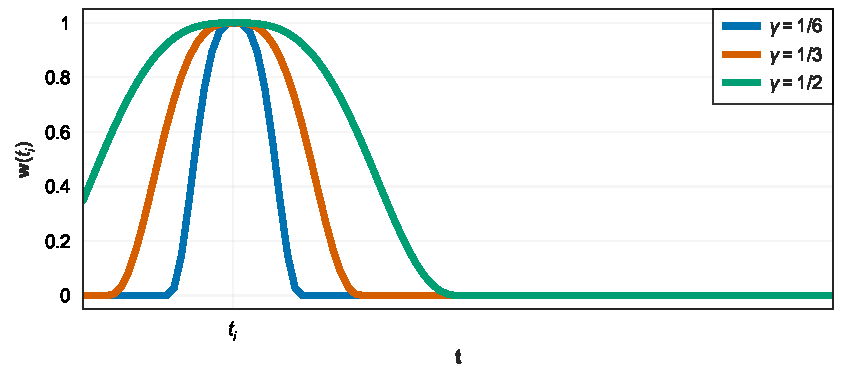
\includegraphics[width=.8\textwidth]{figures/chapter5-lowess/figure1-window.pdf}
	\caption[LOWESS tricube weighting function]{
		LOWESS tricube weighting function $ \bm{w}(t_i) $ for an inclusion fraction of $ \gamma = 1/6 $ (blue), $ \gamma = 1/3 $ (orange), and $ \gamma = 1/2 $ (green).
	}
	\label{fig:ch5-algo-window}
\end{figure}


We can adaptively filter the noisy $ \bm{\phi} $ time series by implementing a robust LOWESS regression \citep{Cleveland1979RobustLocallyWeighted}. The LOWESS algorithm fits a local linear regression at every $t_i$ using nearby data points, repeating over multiple iterations to refine the fit and reduce the effect of outliers \citep{Efron2019ComputerAgeStatistical}.
% which performs several iterations of weighted linear regression for each SAR acquisition. 
For the first iteration, at each time $t_i$,  we calculate a set of weights $\bm{w}(t_i)$. The weight function has a maximum value of $1$ at $t_i$ and decays to zero at the $r$th nearest neighbor to $t_i$, where $r = \left\lfloor \gamma N \right\rfloor$, $0 < \gamma \leq 1$ is the fraction of the data chosen to include for each local fit, and $ \left\lfloor x \right\rfloor $ is rounds $ x $ down to the next lowest integer.
Let $h_i$ be the $r$th smallest number of $\left| x_i - x_k \right|$ for $ k = 0, \ldots, N-1 $.
The $k$th weight $w_k(t_i)$ is defined as
\begin{equation}
	w_k(t_i) = 
	\begin{cases}
		\left( 1 - \left|\frac{t_i - t_k}{h_i} \right|^3 \right)^3 , & \text{if}\  \left|\frac{t_i - t_k}{h_i} \right| < 1 \\
		0, & \text{otherwise}
	\end{cases}          \label{eq:ch5-lowess-weights}
\end{equation}
for $k =0, \ldots, N-1 $. This weight function is known as the \emph{tricube} weighting function.
Figure \ref{fig:ch5-algo-window} illustrates the shape of  $ \bm{w}(t_i) $ for $\gamma = 1/6, 1/3$ and  $1/2 $.



Using $ \bm{w}(t_i) $, we compute a weighted linear regression around $t_i$ by finding the intercept and slope, $a_i, b_i$ that minimize
%\begin{equation}
%		\begin{bmatrix}
%		1, t_0 \\
%		1, t_1 \\
%		\ldots \\
%		1, t_{N-1} \\
%	\end{bmatrix}
%	\begin{bmatrix}
%		a_i \\ b_i
%	\end{bmatrix}
%= \bm{\phi}
%\end{equation}
\begin{equation}
	\sum_{k=0}^{N-1} w_k(t_i) \left(\phi_k - a_i - b_i t_k \right)^2
\end{equation}
The smoothed estimate $\hat{\phi}_i$ at the point $t_i$ is calculated as $\hat{\phi}_i = a_i + t_i b_i$. This process is repeated for all $t_i$,  $i = 0, \ldots, N-1$.

The second iteration performs another weighted least squares fit, this time further downweighting based on the residuals of the first iteration.
Let $\epsilon_k = \left| \hat{\phi}_k - \phi_k  \right|$ be the residual at $t_k$ and $s$ be the median residual for all $k$. We create an additional set of weights $ \delta_k $ for each $ k = 0, \ldots, N-1$ as
\begin{equation}
	\delta_k = 
	\begin{cases}
		\left( 1 - \left(\frac{ \hat{\phi}_k - \phi_k }{6 s} \right)^2 \right)^2 , & \text{if}\  \left( \frac{ \hat{\phi}_k - \phi_k }{6s} \right) < 1 \\
		0, & \text{otherwise}
	\end{cases}          \label{eq:ch5-lowess-weights2}
\end{equation}
Equation \eqref{eq:ch5-lowess-weights2} uses the median $ s $ so that large outliers are clipped to 0, similar to the use of the median absolute deviation from Section \ref{sec:ch4-outlier-method}. For each new fit in the second iteration, the weights $ \bm{w}(t_i) $ are multiplied by the residual weights $\bm{\delta}$ to perform the local regressions.

Finally, we perform a shift of $ \bm{\hat{\phi}} $ to compensate for the first day's atmospheric conditions by setting $ \hat{\phi}_i = \hat{\phi}_i - \hat{\phi}_0 $ for all $ i = 1, \ldots, N-1 $.
This step is necessary for $ \bm{\phi} $ solved using the SBAS formulation of Equation \eqref{eq:ch2-sbas-A}; since the first date's phase is assumed to be 0, $ \alpha_0 $ is added to all other dates.
While \cite{Ferretti2000NonlinearSubsidenceRate} uses mean value of the common-reference interferogram phases as an estimation of the first date's atmospheric noise, here we use the y-intercept of the smoothed time series, $ \hat{\phi}_0 $, as an estimate of $ \alpha_0 $. 


%
%%$ \bm{v} = (\bm{A}^T \bm{A})^{-1}\bm{A}^T \bm{\Delta \phi} $
%%As noted in \cite{Simons2007InterferometricSyntheticAperture}, 
%The least squares solution $ \bm{v} = (\bm{B}^T \bm{B})^{-1}\bm{B}^T \bm{\Delta \phi} $ (or minimum norm solution n $ \bm{v} = \bm{B}^{\dagger} \bm{\Delta \phi}$ ) from \cite{Berardino2002NewAlgorithmSurface} assume that all measurements in $\bm{\Delta \phi}$ have equal variance; subsequent authors have implemented a weighted least squares solution:
%\begin{equation}
%	%	\bm{\phi} = \bm{A}^{\dagger} \bm{\Delta \phi}
%	%	\bm{\phi} = (\bm{A}^T \bm{\Sigma}^{-1} \bm{A})^{-1}\bm{A}^T \bm{\Sigma}^{-1} \bm{\Delta \phi}  \label{eq:ch2-sbas-wls}
%	\bm{v} = (\bm{B}^T \bm{\Sigma}^{-1} \bm{B})^{-1}\bm{B}^T \bm{\Sigma}^{-1} \bm{\Delta \phi}  \label{eq:ch2-sbas-wls}
%\end{equation}
%where $ \bm{\Sigma} = \mathbb{E}[\bm{\epsilon} \bm{\epsilon}^T] $ is the measurement covariance matrix.


\section{Synthetic Example}

\begin{figure}[!h]
	\centering
%	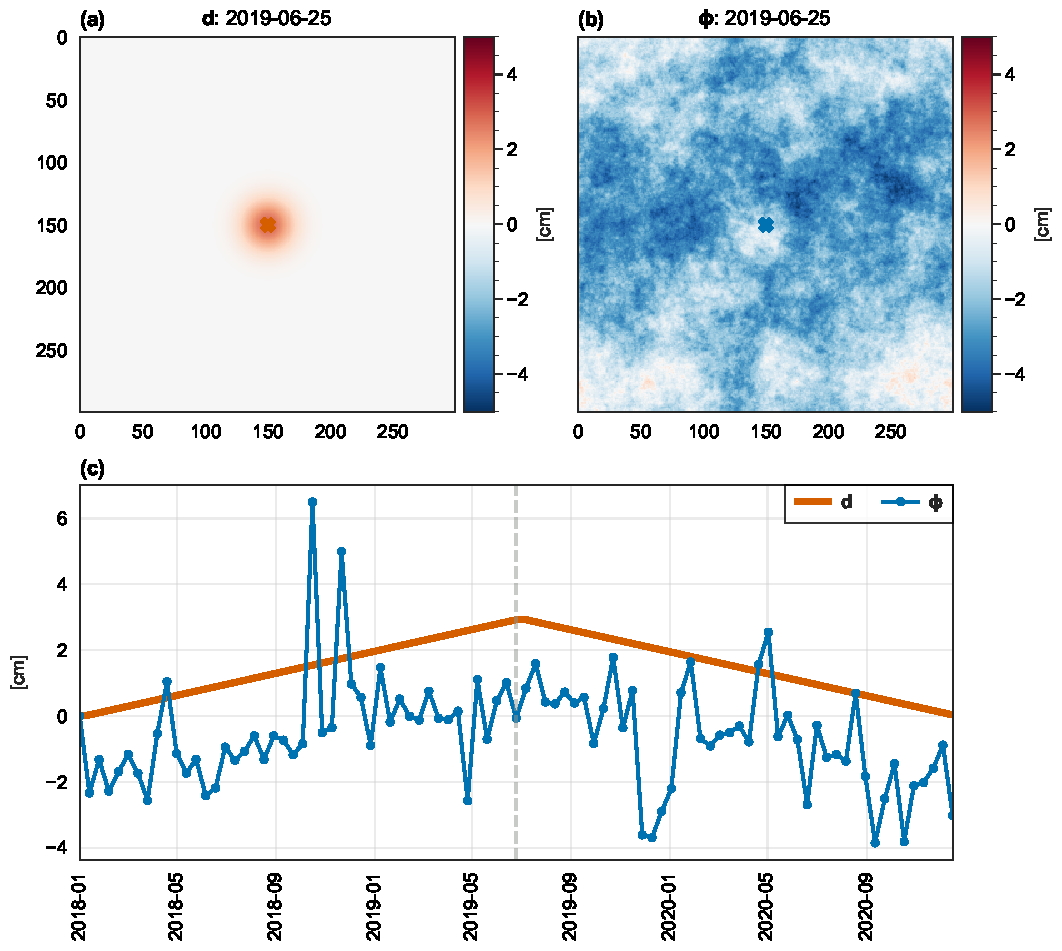
\includegraphics[width=.99\textwidth]{figures/chapter5-lowess/figure2-demo-data.pdf}
	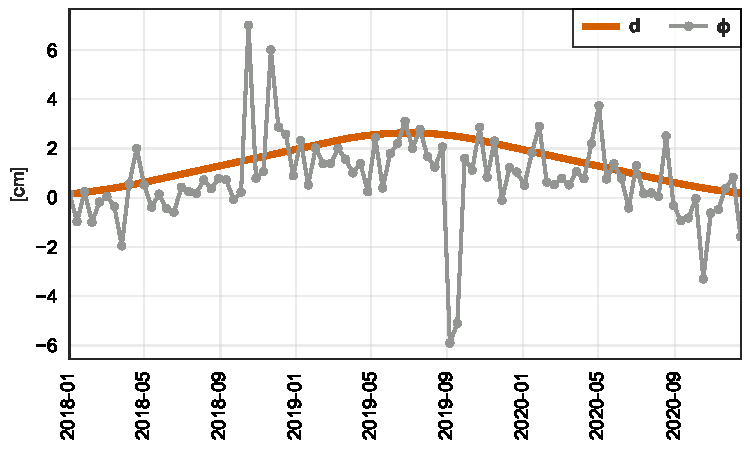
\includegraphics[width=.75\textwidth]{figures/chapter5-lowess/figure2-demo-data-ts-only.pdf}
	\caption[Synthetic data for LOWESS smoothing]{
%		(a)  A 300 x 300 pixel region contains a synthetic uplift bowl which peaks at 3 cm.
%		(b) Turbulent tropospheric is noise added to panel (a) for 
%		(c) 
		Synthetic time series for one pixel $ \bm{\phi} $ (gray) containing a combination of true deformation $\bm{d}$ (orange) and non-Gaussian tropospheric noise $ \bm{\alpha} $: $\bm{\phi} =\bm{d} + \bm{\alpha}$. 
%		The pixel marked with an x in panels (a) and (b) shows the location of the $\bm{d}$ and $\bm{\phi}$ time series, respectively.
%		The date shown in panels (a) and (b) is marked with the grey dashed line. 
		Note that the $ \bm{\phi} $ time series is offset by an amount equal to the noise on the first date, due to the SBAS assumption that $ \phi_0 = 0 $.
	}
	\label{fig:ch5-demo-data}
\end{figure}


We first illustrate the LOWESS algorithm on a synthetic 3-year deformation time series with a 12-day acquisition interval (Figure \ref{fig:ch5-demo-data}).
%A 300 x 300 pixel region contains an uplift bowl which linearly increases to $ \sim3 $cm max after 1.5 years (Figure \ref{fig:ch5-demo-data}a) and deflates back to zero by the end of 3 years. 
The true deformation linearly increases to maximum of $ \sim3 $cm after 1.5 years and deflates back to zero by the end of 3 years. 
Non-Gaussian noise containing jumps of up to 8 cm is added to the deformation.
%similar to tropospheric noise is simulated following \cite{Hanssen2001RadarInterferometryData} and 
% (Figure \ref{fig:ch5-demo-data}b). 
%The uplift bowl inflates at a constant rate for 1.5 years, then deflates back to 0 by the end of the 3rd year (Figure \ref{fig:ch5-demo-data}c).
%To simulate the output from an SBAS inversion, 
The time series is shifted by the noise on the first day so that $ \phi_0 = 0 $, simulating the result from an SBAS inversion.



\begin{figure}
	\centering
	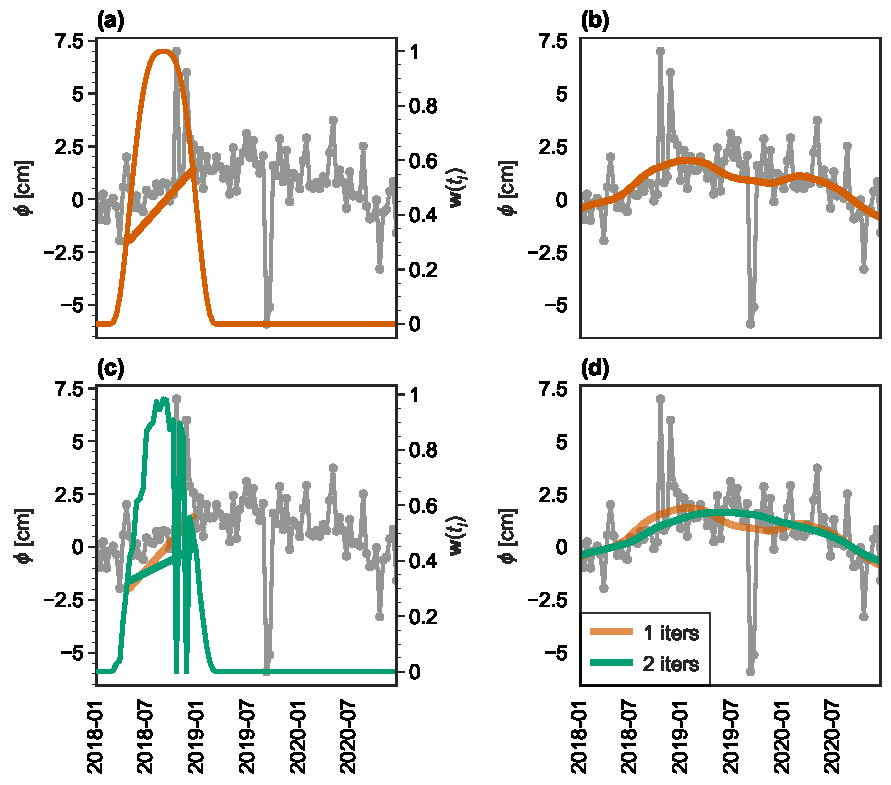
\includegraphics[width=.95\textwidth]{figures/chapter5-lowess/figure3-fits.pdf}
	\caption[Demo of LOWESS fitting]{
		(a) First iteration of local fit at $t_i$, weighted by window (orange) with $ \gamma=0.4 $ ($ \sim $1.2 year of data). 
%		Shading of dots indicates the weight factor, where gray indicates 0 weighting and gold indicates full weighting.
		(b) First iteration of smoothed $ \hat{\phi}_i $ (orange line) for all $i$. 
		(c) Second iteration at $t_i$ with the updated residual weighting. The large anomalous points have a smaller effect on the new local fit (green slope) compared to the original (orange slope).
		% to produce a new weighted least squares fit.
		(d) Result of second iteration of LOWESS smoothing for all $i$ (green line).
	}
	\label{fig:ch5-algo-demo}
\end{figure}



Figure \ref{fig:ch5-algo-demo} illustrates two iterations of the LOWESS algorithm the $ \bm{\phi} $ time series.
During the first iteration, each $ \hat{\phi}_i $ is calculated using a locally weighted regression with the weight based solely on the proximity to $ t_i $ (Figure \ref{fig:ch5-algo-demo}a). The resulting fit tracks the general pattern of the data, but outlier points strongly influence the fit (Figure \ref{fig:ch5-algo-demo}b). 
%Using the residuals of the fit from Figure \ref{fig:ch5-algo-demo}b, 
The second iteration multiplies the proximity weighting from Figure \ref{fig:ch5-algo-demo}a by the residual weighting, $ \bm{\delta} $, calculated from the previous iteration (Figure \ref{fig:ch5-algo-demo}c).
The second iteration is influenced less by the outlier points and has fewer spurious bumps in the time series (Figure \ref{fig:ch5-algo-demo}d). In general, more iterations may be performed; in this example, further iterations change the fit by $ \sim $ 1 mm or less.



\begin{figure}[!h]
	\centering
%	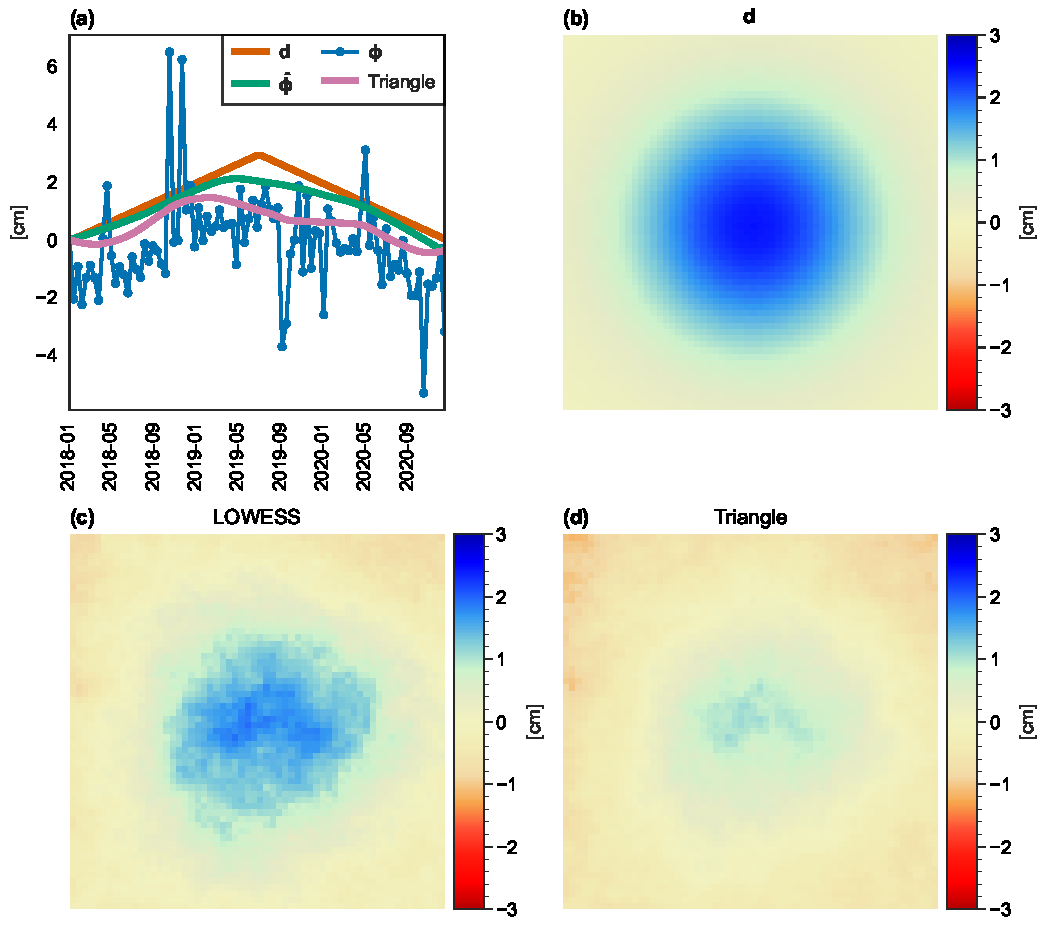
\includegraphics[width=.99\textwidth]{figures/chapter5-lowess/figure4-compare-tri.pdf}
	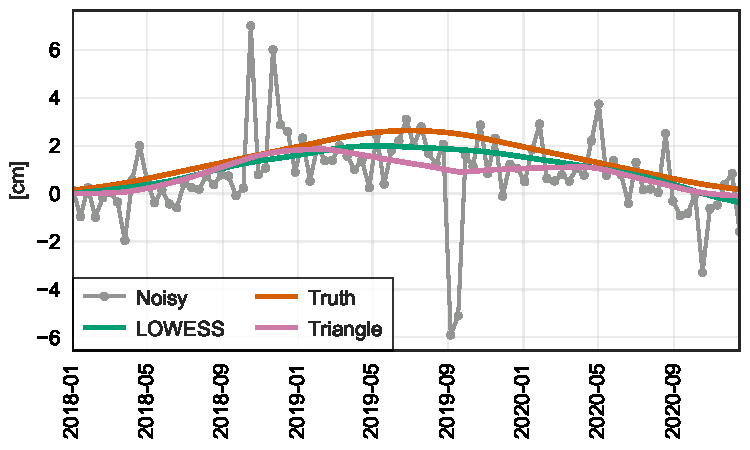
\includegraphics[width=.75\textwidth]{figures/chapter5-lowess/figure4-compare-tri-ts-only.pdf}
	\caption[Comparison of LOWESS smoothing to triangle filter for synthetic data]{
		Results of smoothing the synthetic noisy time series $ \bm{\phi} $ (gray with dots) using the LOWESS algorithm (green) and a triangle filter (pink). True deformation time series is shown in orange. Both the LOWESS algorithm and the triangle filter use $ 40 $\% of the data (a filter width of $ \sim $1.2 years) and have been shifted to compensate the first day's atmospheric noise.
}
	\label{fig:ch5-compare-tri}
\end{figure}

After subtracting $ \phi_0 $ from all points, the results of the LOWESS estimate $ \bm{\hat{\phi}} $ are shown in Figure \ref{fig:ch5-compare-tri} (green line). The LOWESS algorithm smooths away the large spikes of turbulence noise in  $ \bm{\phi} $ (Figure \ref{fig:ch5-compare-tri}, gray) and captures most of the deformation signal (Figure \ref{fig:ch5-compare-tri}, orange)
%We note that since the width of the weighting window $ \bm{w} $ was slightly over 1 year, the algorithm smooths over the peak of the deformation lasting several months (Figure \ref{fig:ch5-compare-tri}a, orange line),
%The LOWESS solution captures most of the deformation signal (Figure \ref{fig:ch5-compare-tri}c), missing only the sharp peak due to the 1.2 year weighting window.
For comparison, we have also linearly filtered the noisy time series with triangle filter of width 1.2 years (Figure \ref{fig:ch5-compare-tri} pink line). 
The triangle filter performs similarly to LOWESS when the noise is Gaussian; however, the large turbulence jumps in this example cause the triangle filter to be pulled $>2$ cm away from the true deformation time series.





\section{7-year Sentinel-1 cumulative surface deformation}

We demonstrate the LOWESS algorithm on real Sentinel-1 data over the Permian Basin.
We processed an additional three years of data (Jan. 2019 though Dec. 2021) for Path 78 (Figure \ref{fig:paper1-study-area}) following the processing strategy outlined in Section \ref{sec:ch3-insar-processing}, for a total of 151 SAR acquisitions from Nov. 2014 to Dec. 2021
We performed an unregularized SBAS inversion to get a noisy time series $ \bm{\phi} $ for each pixel. 
To mitigate residual long wavelength noise from seasonal tropospheric patterns, we fit and removed a quadratic surface from the deformation map at each SAR acquisition using pixels with $<$2 cm of estimated deformation \citep{Morishita2020LicsbasOpenSource}. We then temporally smoothed each pixel's using the LOWESS algorithm with a weighting window covering $\geq 2$ years at all time intervals and 2 robust iterations. We similarly processed 147 descending Path 85 SAR acquisitions to create a 7-year cumulative LOS deformation time series.

% sampled every 6 months.
We also processed 148 SAR acquisitions from ascending Path 151 (west of Path 85) to cover the full Delaware Basin with at least $2$ paths of data in all location.
The Path 151 footprint does not contain GPS station TXKM that was used as the reference location for the other paths;
%therefore, or any other GPS station near the center of the footprint, 
instead, we used the technique presented in \cite{Zebker2021AccuracyModelFree} to fit and remove a phase-elevation trend from all high-coherence pixels in each interferogram and zero-reference the deformation. This method is effective for study areas where only a subset of high-coherence interferogram pixels contain significant deformation.
%. which is true for Path 151 which only partially overlaps with the Permian Basin's production region.

\subsection{GPS comparison and smoothing window choice}
\label{sec:ch5-results-gps}


\begin{figure}[h]
	\centering
	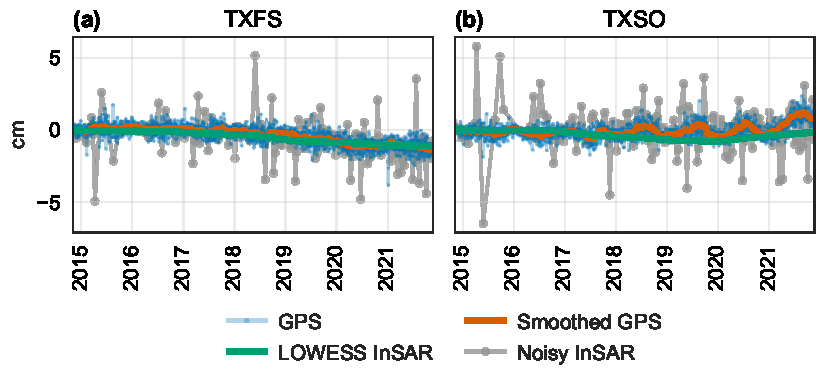
\includegraphics[width=.99\textwidth]{figures/chapter5-lowess/gps_path78_2plots.pdf}
	\caption[Example results for Path 78 LOWESS smoothing]{
		Path 78 LOWESS smoothed algorithm (orange line) plotted against the original noisy time series (gray) at pixels near (a) station TXFS, and (b) station TXSO.
		GPS time series (blue dots) have been projected onto the radar LOS. 
		%		Orange line shows 30 day moving average of GPS daily measurements.
	}
	\label{fig:ch5-results-gps-example}
\end{figure}

To assess the performance of the LOWESS-smoothed LOS deformation results, we projected the available GPS ENU time series onto the radar LOS. 
As an example, Figure \ref{fig:ch5-results-gps-example}a shows the LOS time series (blue dots) for GPS station TXFS.
%, along with its 30-day moving average (orange line).
The unregularized InSAR time series (gray) contains up to 5-7 cm of tropospheric noise during the summer months. However, the LOWESS solution (green line) is unaffected by the spikes and successfully tracks the $ \sim1 $cm of long term motion shown in the GPS data. 
In Figure \ref{fig:ch5-results-gps-example}b, the LOS time series for GPS station TXSO shows a combination of a 5-10 mm increase in LOS along with 10-15 mm of seasonal variations.
While the trend is captured by the InSAR LOWESS solution, the seasonal variations are smoothed over due to the $2$ year weighting window.

We compared multiple choices of the LOWESS window size to determine an appropriate choice of $ \gamma $ which balances the tradeoff between noise reduction and temporal resolution.
To estimate the variance of the LOWESS-smoothed solution, we used the bootstrap technique \citep{Efron1979BootstrapMethodsAnother, Efron1994IntroductionBootstrap}, which have been included in InSAR time series packages such as GIAnT, MintPy, and LiCSBAS
\citep{Agram2013NewRadarInterferometric, Yunjun2019SmallBaselineInsar, Morishita2020LicsbasOpenSource}.
%The bootstrap and jackknife (a special case of the bootstrap) techniques have been included in various InSAR time series packages including GIAnT, MintPy, and LiCSBAS


\begin{figure}[h]
	\centering
	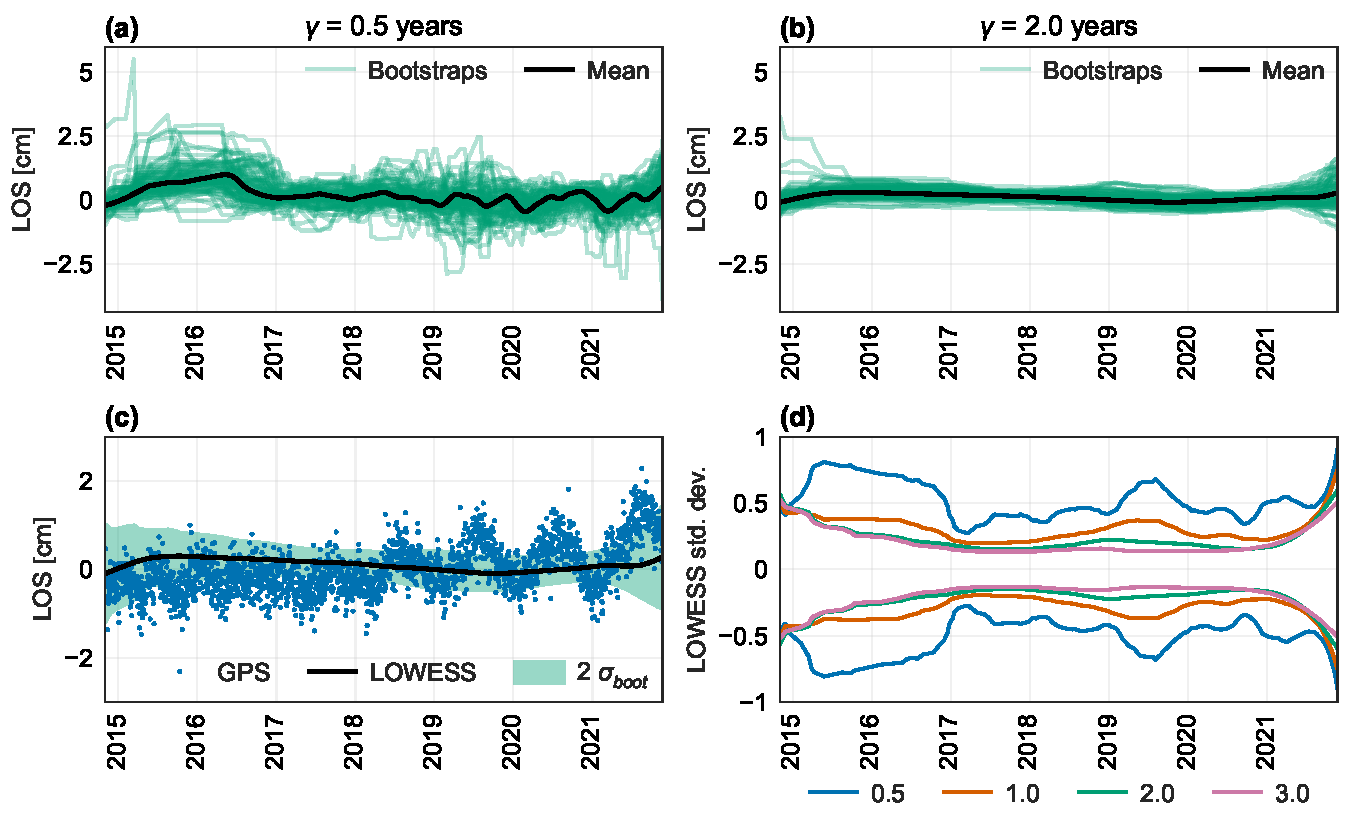
\includegraphics[width=.99\textwidth]{figures/chapter5-lowess/figure-results-bootstrap.pdf}
	\caption[Cumulative 7-year LOS deformation for three Sentinel-1 paths]{
	LOWESS smoothed solutions of bootstrap resampled noisy InSAR time series at GPS station TXSO using a window size of (a) $ \gamma = 0.5 $ and (b) $ \gamma = 2 $ years. Each smoothed resampling is shown as a green line, with the mean of all green lines shown in black.
	(c) LOWESS InSAR solution compared to GPS stations projected onto the radar LOS for the $ \gamma = 2 $ year case. Green shaded region shows $ \pm 2  $ standard deviations as estimated by taking the standard deviation of all resampled solutions from panel (b).
	(d) Bootstrap estimated standard deviation of LOWESS result for $ \gamma = 0.5, 1, 2 $, and $ 3 $ years of smoothing.
	}
	\label{fig:ch5-results-bootstrap}
\end{figure}



Figure \ref{fig:ch5-results-bootstrap} shows an example of the bootstrap analysis on the InSAR data near GPS station TXSO.
We resampled the datapoints from the noisy $ \bm{\phi} $ with replacement and performed the LOWESS smoothing on each bootstrap sample (Figure \ref{fig:ch5-results-bootstrap}b). As the number of bootstrap draws increases, the mean of the LOWESS results (black) converges to the smoothed result on the real data.
Taking the standard deviation of the resamples gives an estimate the variance of the smoothed result (Figure \ref{fig:ch5-results-bootstrap}b).
Note that the $ \gamma = 0.5  $ year solutions have a much larger variance than the $ 2 $ year smoothed solutions; however, the variance starts to converge after a 2 year window (Figure \ref{fig:ch5-results-bootstrap}d). Note that while increasing window size decreases the variance in the middle of the time series, the end points still have the highest uncertainty. Similar to other linear fitting procedures, the uncertainty of the estimated slopes propagate into a larger absolute uncertainty at the end points of the data.

%(d) Bootstrap estimated standard deviation of LOWESS result for $ \gamma = 0.5, 1, 2 $, and $ 3 $ years of smoothing.


The full set of GPS comparisons for Path 78 is shown in Figure \ref{fig:ch5-results-gps}. 
The additional 3 years of Sentinel-1 data allow for an additional two station comparisons (at TXM5, TXB8) for a total of 15 stations within the Path 78 footprint.
There is an average of 3 mm RMS difference between the smoothed GPS time series and the InSAR LOWESS solutions for all time steps across the 15 stations, and a maximum absolute difference of 1.3 cm at any time point (including seasonal variations).

%TODO: discuss the end point variance? largest uncertainty for the final 6-12 months?

\begin{figure}
	\centering
%	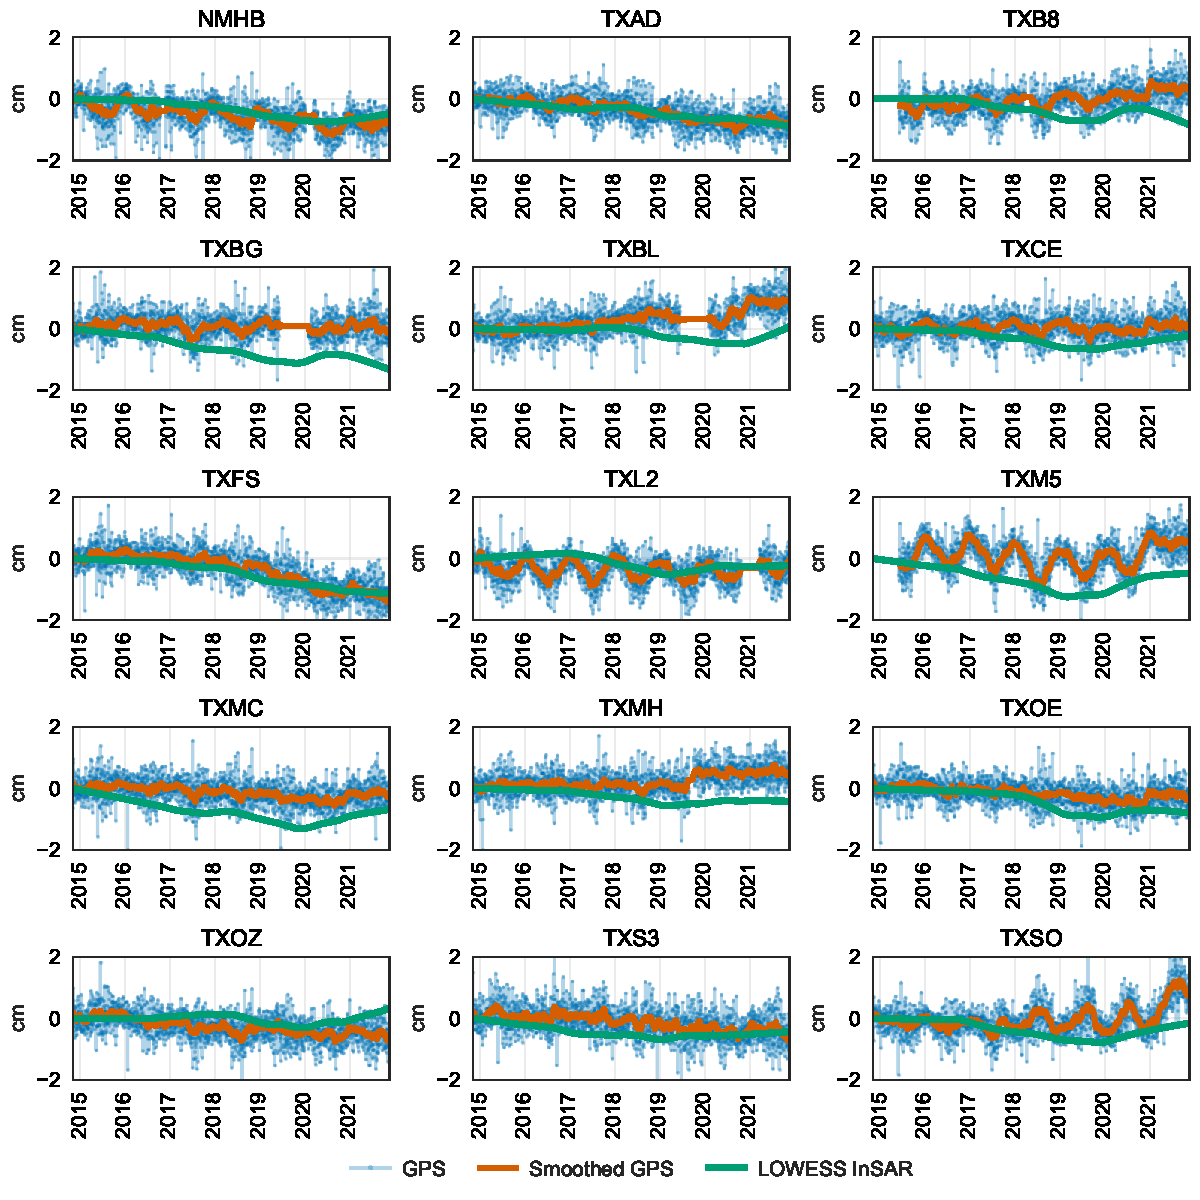
\includegraphics[width=.99\textwidth]{figures/chapter5-lowess/gps_path78.pdf}
	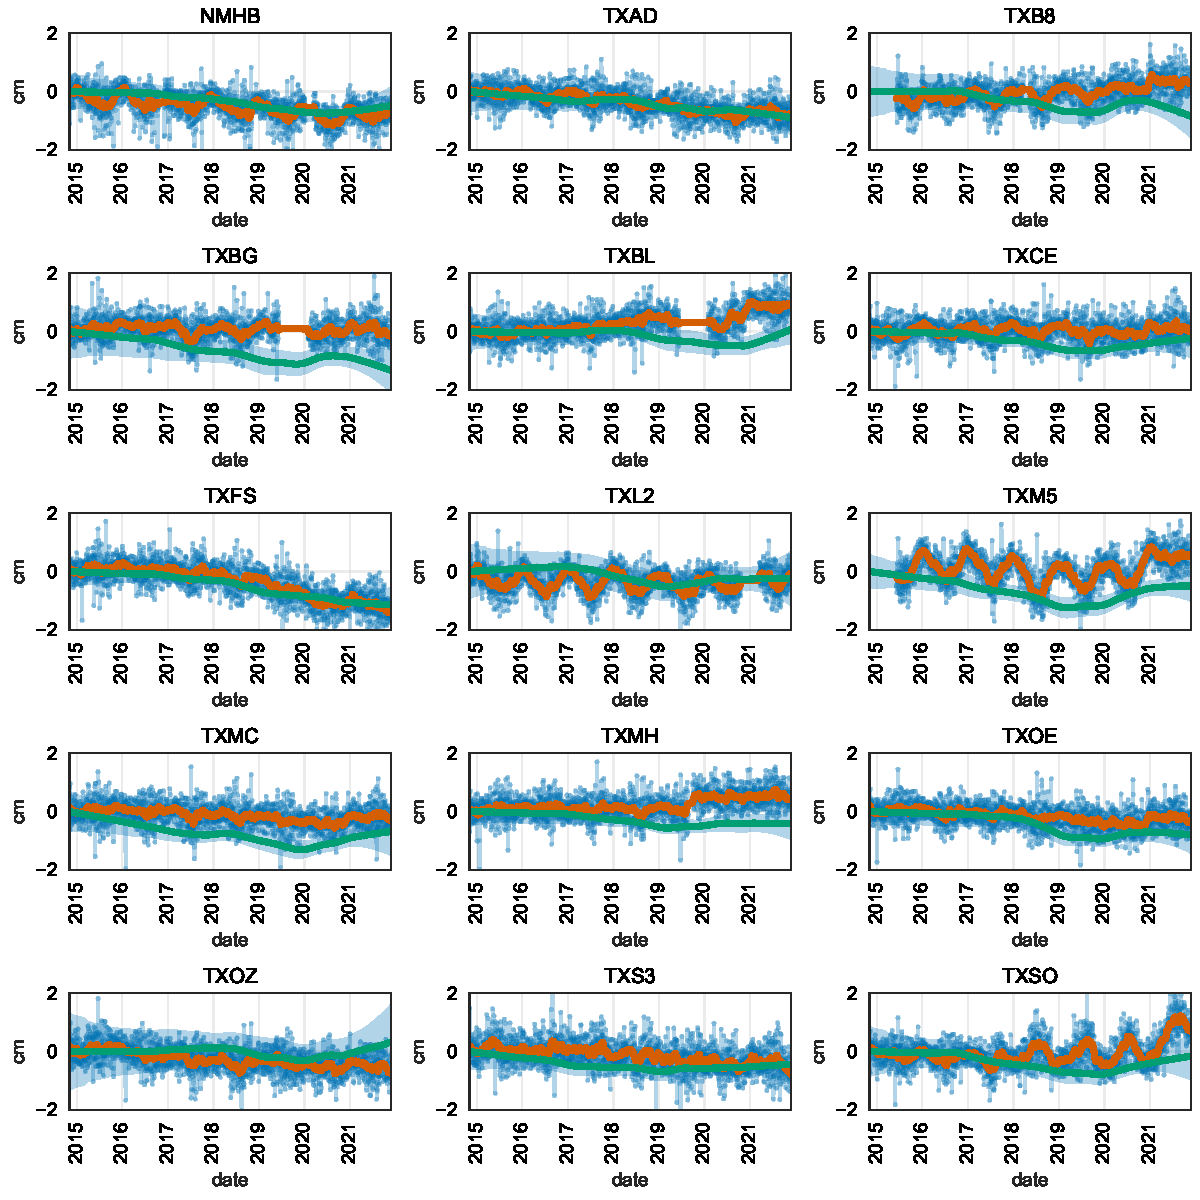
\includegraphics[width=.99\textwidth]{figures/chapter5-lowess/gps_path78_with_sigma.pdf}
	\caption[Full GPS comparison for Path 78 LOWESS solutions]{
		Comparison of permanent GPS stations projected onto the radar LOS (blue dots)
		with Path 78 LOWESS smoothed algorithm (orange lines). Green shaded region shows $ \pm 2  $ standard deviations as estimated by bootstrap resampling.
%		Orange lines show 30 day moving average of GPS daily measurements.
	}
	\label{fig:ch5-results-gps}
\end{figure}

\FloatBarrier




\subsection{LOS deformation results}
\label{sec:ch5-results-path78}

\begin{figure}
	\centering
	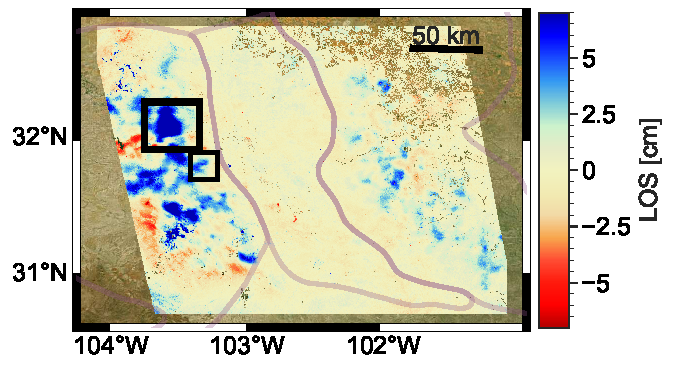
\includegraphics[width=.99\textwidth]{figures/chapter5-lowess/figure-results-los-path78.pdf}
	\caption[Cumulative 7-year LOS deformation for three Sentinel-1 paths]{
		Cumulative LOS deformation from Nov. 2014 to Dec. 2021 for ascending 78. Blue areas indicate motion away from the satellite (subsidence or eastward). Areas with low correlation have been masked.
		Black boxes indicate the zoomed-in locations for Figure \ref{fig:ch5-results-path78-examples} panels (a) and (c).
		Purple outlines indicate (from west to east) the Delaware Basin, Central Basin Platform, and Midland Basin.
	}
	\label{fig:ch5-results-path78}
\end{figure}

\begin{figure}
	\centering
	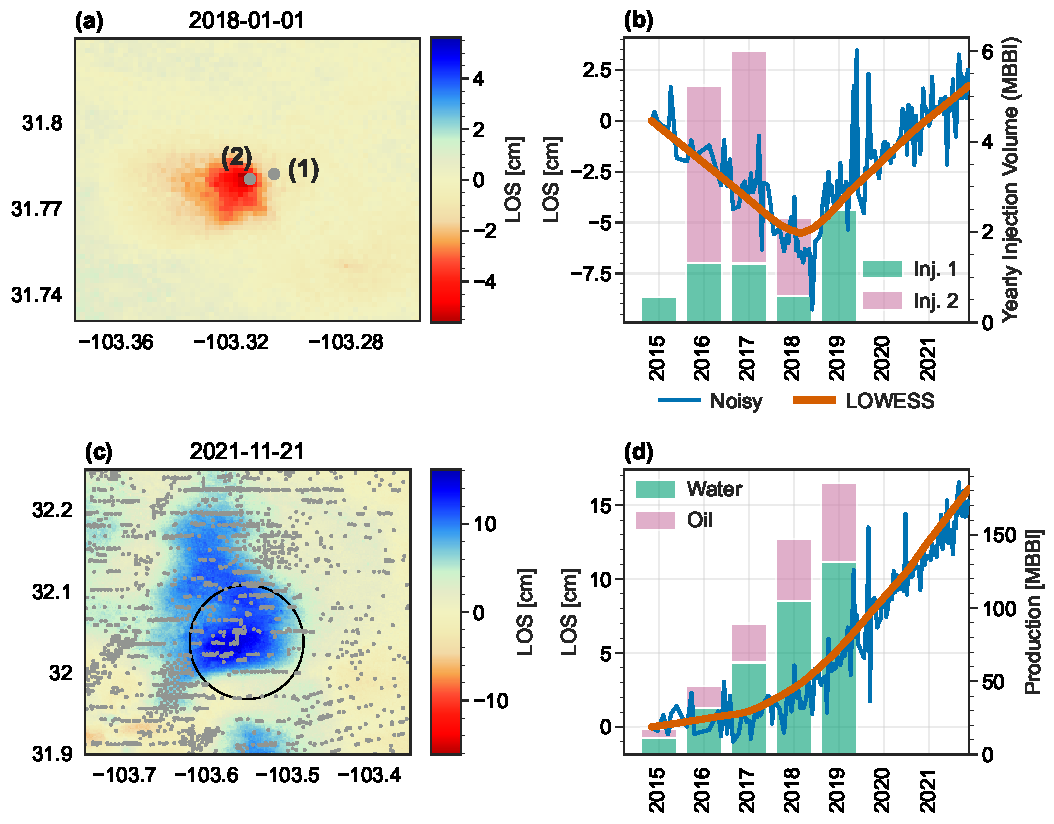
\includegraphics[width=.99\textwidth]{figures/chapter5-lowess/figure-results-path78-examples.pdf}
	\caption[Path 78 deformation features]{
		(a) Cumulative LOS deformation for ascending Path 78 through Jan. 2018 using LOWESS smoothing algorithm. Red (negative LOS) indicates motion toward the satellite. 
		Grey dots show the locations of two nearby Texas salt water disposal wells (Well 1: API 49530150, Well 2: API 49533675).
		(b) Time series of pixel location of maximum uplift in panel (a) showing noisy $ \bm{\phi} $ (blue) and LOWESS result (orange). Green and pink bars show the annual injection volume of wells 1 and 2, respectively, indicating that Well 2 shut down injection operations after 2018.
		(c) Cumulative LOS deformation for ascending Path 78 from Nov. 2014 to Dec. 2021. Grey dots indicate the location of oil or water production wells that were active between 2014 and 2019.
		(d) Noisy SBAS time series (blue) and smoothed LOWESS result (orange) for InSAR pixel in the center of the circle in panel (c).
		Annual production volumes of water (green) and oil (pink) for all wells contained in circle of panel (c). Note that production continued into 2020 and 2021, but individual well data was unavailable.
	}
	\label{fig:ch5-results-path78-examples}
\end{figure}

Figure \ref{fig:ch5-results-path78} shows the 7-year cumulative LOS deformation map for Path 78, where areas with low average spatial coherence ($ < 0.2 $) or temporal coherence $ < 0.75 $ are masked. 
%The shows similar patterns present in the 2015-2018 map from Section \ref{sec:ch4-results-defo}. 
%(Figure \ref{fig:ch4-insar-los})
%While most subsidence bowls in the Midland Basin were $ \sim1-3 $ cm in magnitude in Jan. 2019, many have increased to $ > 6 $ cm by Dec. 2021.
% most subsidence bowls in the Midland Basin were $ \sim1-3 $ cm in magnitude in Jan. 2019, many have increased to $ > 6 $ cm by Dec. 2021.
%However, there are several notable deformation rate changes between the 2015-2018 period and the 2019-2021 period.
While many spatial patterns present in the map are also visible in the 4-year deformation map (Figure \ref{fig:ch4-insar-los}), there are several notable deformation rate changes between the 2015-2018 period and the 2019-2021 period.
For example, near the SWD wells identified in \cite{Kim2018AssociationLocalizedGeohazards} (Figure \ref{fig:ch5-results-path78-examples}a), there was steady surface uplift as injection volume increased from 2015-2018. After the injection well near the uplift peak (Well 2) shut down operations after 2018, there was a gradual deflation for the next three years (Figure \ref{fig:ch5-results-path78-examples}b).
In the northern Delaware Basin, many of the subsidence patterns present in the 4-year cumulative maps show accelerating rates of subsidence as oil production volumes increased through 2020.
One example subsidence bowl on the New Mexico side of the TX-NM border (Figure \ref{fig:ch5-results-path78-examples}c) subsided 4-5 cm for the four years of 2015-2018. As both oil and water production increased in the surrounding wells, the subsidence rate increased to $ >5 $ cm per year.



%
%\begin{figure}
%	\centering
%	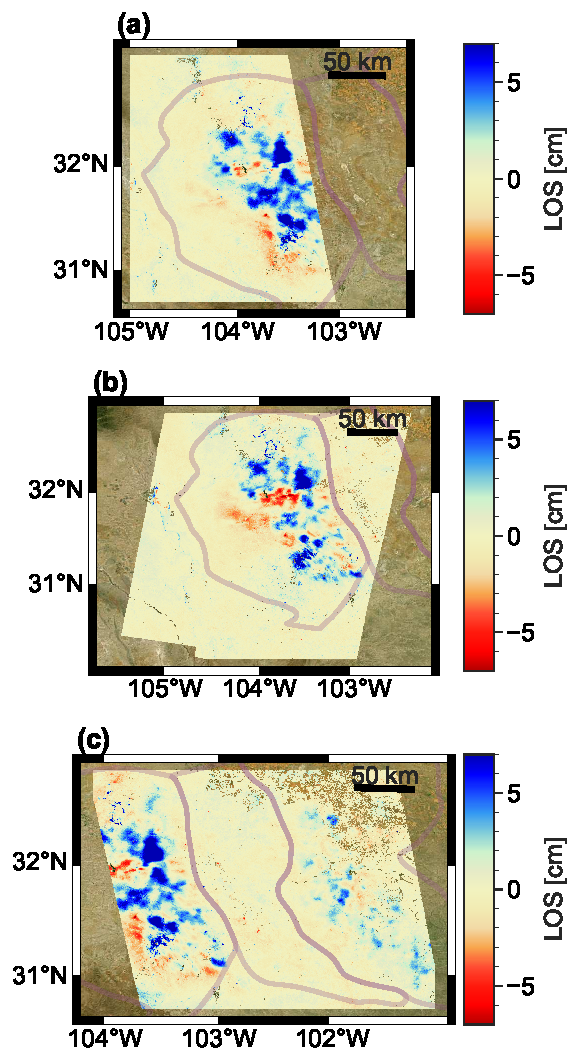
\includegraphics[height=.9\textheight]{figures/chapter5-lowess/figure-results-los.pdf}
%	\caption[Cumulative 7-year LOS deformation for three Sentinel-1 paths]{
%		Cumulative LOS deformation from Nov. 2014 to Dec. 2021 for (a) ascending Path 151, (b) descending Path 85, and (c) ascending Path 78.  Blue areas indicate motion away from the satellite, areas with low correlation have been masked.
%		Purple outlines indicate (from west to east) the Delaware Basin, Central Basin Platform, and Midland Basin.
%	}
%	\label{fig:ch5-results-los}
%\end{figure}


%
%\begin{figure}
%	\centering
%	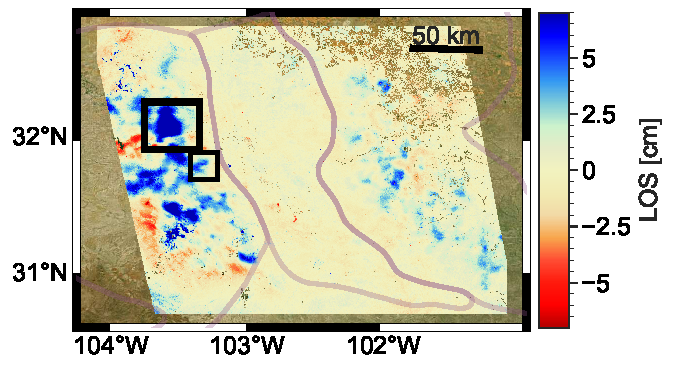
\includegraphics[width=.99\textwidth]{figures/chapter5-lowess/figure-results-los-path78.pdf}
%	\caption[Path 78 cumulative deformation]{
%		(a) Cumulative LOS deformation for ascending Path 78 from Nov. 2014 to Dec. 2021 using LOWESS smoothing algorithm. Red (negative LOS) indicates motion toward the satellite. Pixels with low correlation have been masked.
%		(b) Time series of pixel indicated by black box in panel (a) near location of former waste water injection well (Figure \ref{fig:ch2-injection-kim-lu}) showing noisy $ \bm{\phi} $ time series (blue) and LOWESS result (orange).
%		Green bars show the annual injection volume of nearby Texas salt water disposal well (API  49533675).
%	}
%	\label{fig:ch5-results-path78}
%\end{figure}
%
%
%\begin{figure}
%	\centering
%	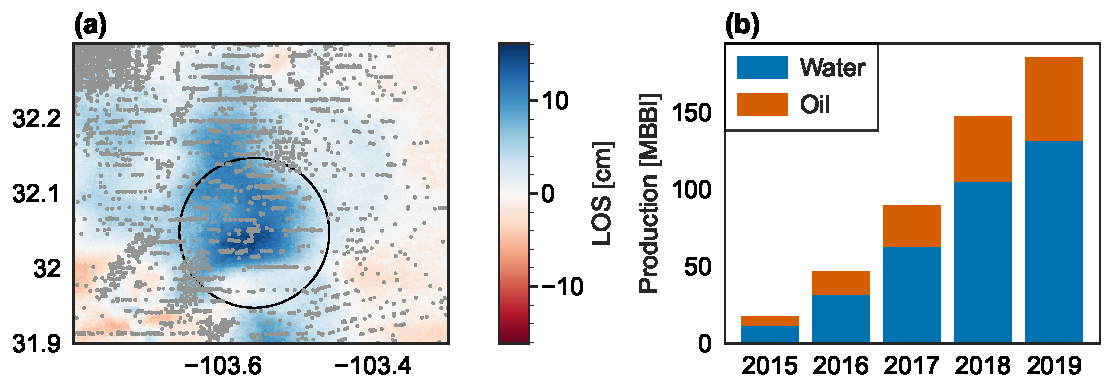
\includegraphics[width=.99\textwidth]{figures/chapter5-lowess/figure-los-path78-production.pdf}
%	\caption[Cumulative deformation near oil and water production]{
%		(a) Cumulative LOS deformation for ascending Path 78 from Nov. 2014 to Dec. 2021. Blue areas contain subsidence from oil and water production. Grey dots indicate the location of wells active between 2014 and 2019.
%		(b) Annual production volumes of water (blue) and oil (orange) for all wells contained in circle of panel (a).
%	}
%	\label{fig:ch5-results-path78-subs}
%\end{figure}



\begin{figure}
	\centering
%	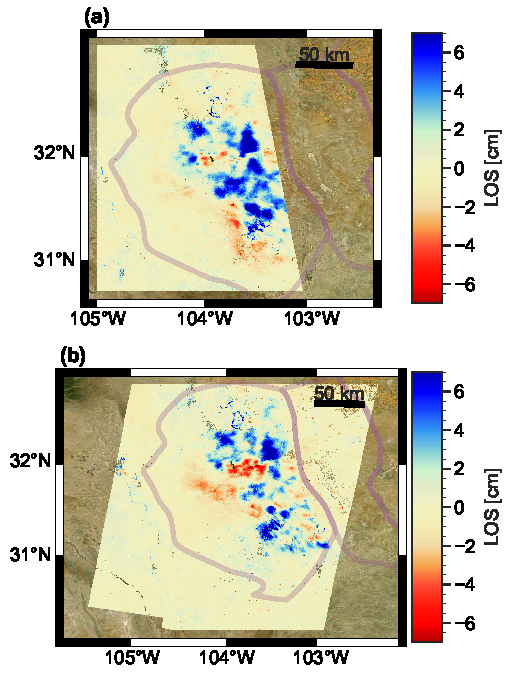
\includegraphics[height=.9\textheight]{figures/chapter5-lowess/figure-results-los-paths-85-151.pdf}
	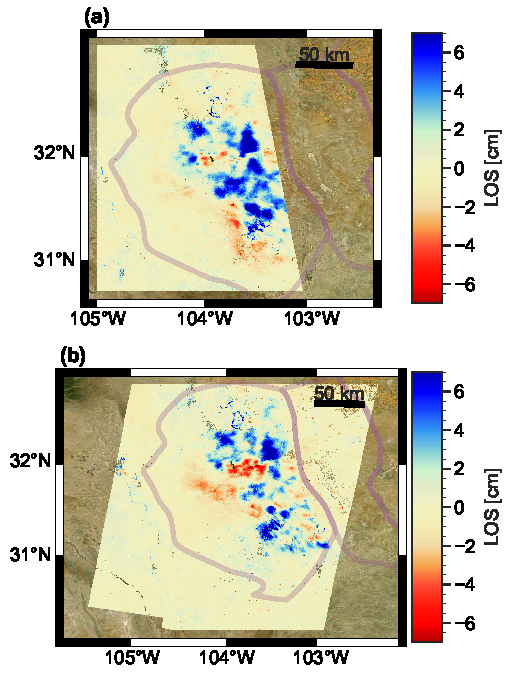
\includegraphics[width=.9\textwidth]{figures/chapter5-lowess/figure-results-los-paths-85-151.pdf}
	\caption[Cumulative 7-year LOS deformation for Paths 85 and 151]{
		Cumulative LOS deformation from Nov. 2014 to Dec. 2021 for (a) ascending Path 151 and (b) descending Path 85.  Blue areas indicate motion away from the satellite, areas with low correlation have been masked.
		Purple outlines indicate (from west to east) the Delaware Basin, Central Basin Platform, and Midland Basin.
	}
	\label{fig:ch5-results-los-paths-85-151}
\end{figure}



\FloatBarrier
%\subsection{Vertical Deformation}

The cumulative LOS deformation from Nov. 2014 to Dec. 2021 is shown in Figure \ref{fig:ch5-results-los-paths-85-151} for Path 151 (panel (a)), and Path 85 (panel (b)).
In addition to the LOS decomposition using Paths 78 and 85 described in Section \ref{sec:ch4-insar-decomp}, we performed a second LOS decomposition using Paths 85 and 151.
We merged the two decompositions by averaging their region of overlap, and we cropped the maps to the western contour of the Delaware Basin to obtain continuous vertical (Figure \ref{fig:ch5-results-east-up}a) and eastward (Figure \ref{fig:ch5-results-east-up}b) deformation solutions.


\begin{figure}
	\centering
%	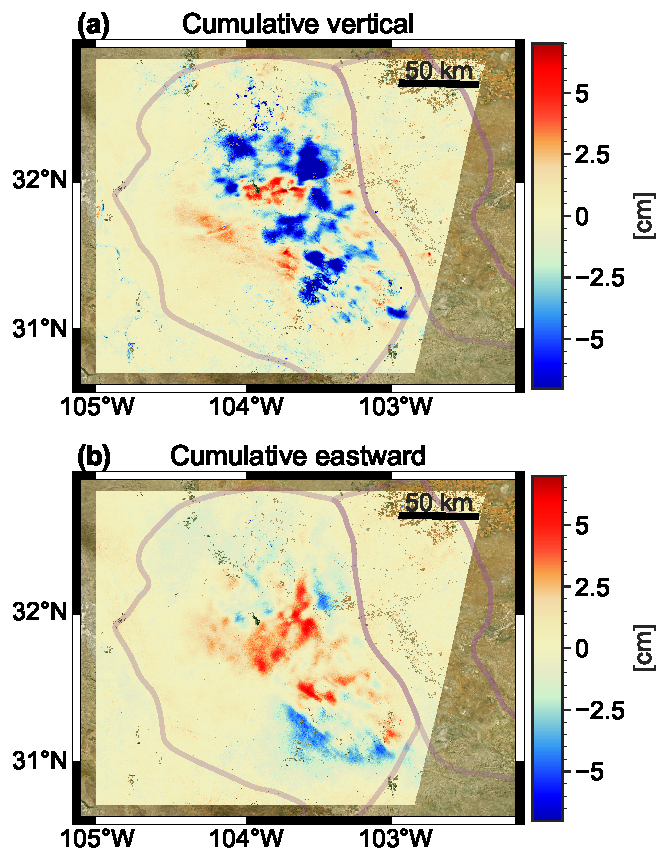
\includegraphics[height=.9\textheight]{figures/chapter5-lowess/figure-results-east-up.pdf}
	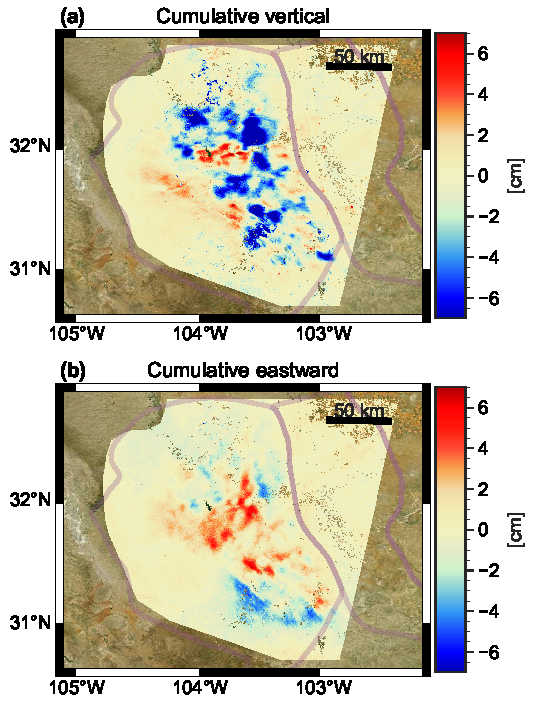
\includegraphics[height=.9\textheight]{figures/chapter5-lowess/figure-results-east-up-clipped.pdf}
	\caption[Cumulative 7-year vertical and eastward deformation]{
		Cumulative (a) vertical and (b) eastward deformation from Nov. 2014 to Dec. 2021. Blue areas indicate subsidence (westward motion), red indicates uplift (eastward). Purple outlines indicate the Delaware Basin (to the west) and Central Basin Platform (east).
	}
	\label{fig:ch5-results-east-up}
\end{figure}



%\section{Discussion}

%The cumulative vertical surface deformation (Figure \ref{fig:ch5-results-east-up}a)




\begin{figure}
	\centering
	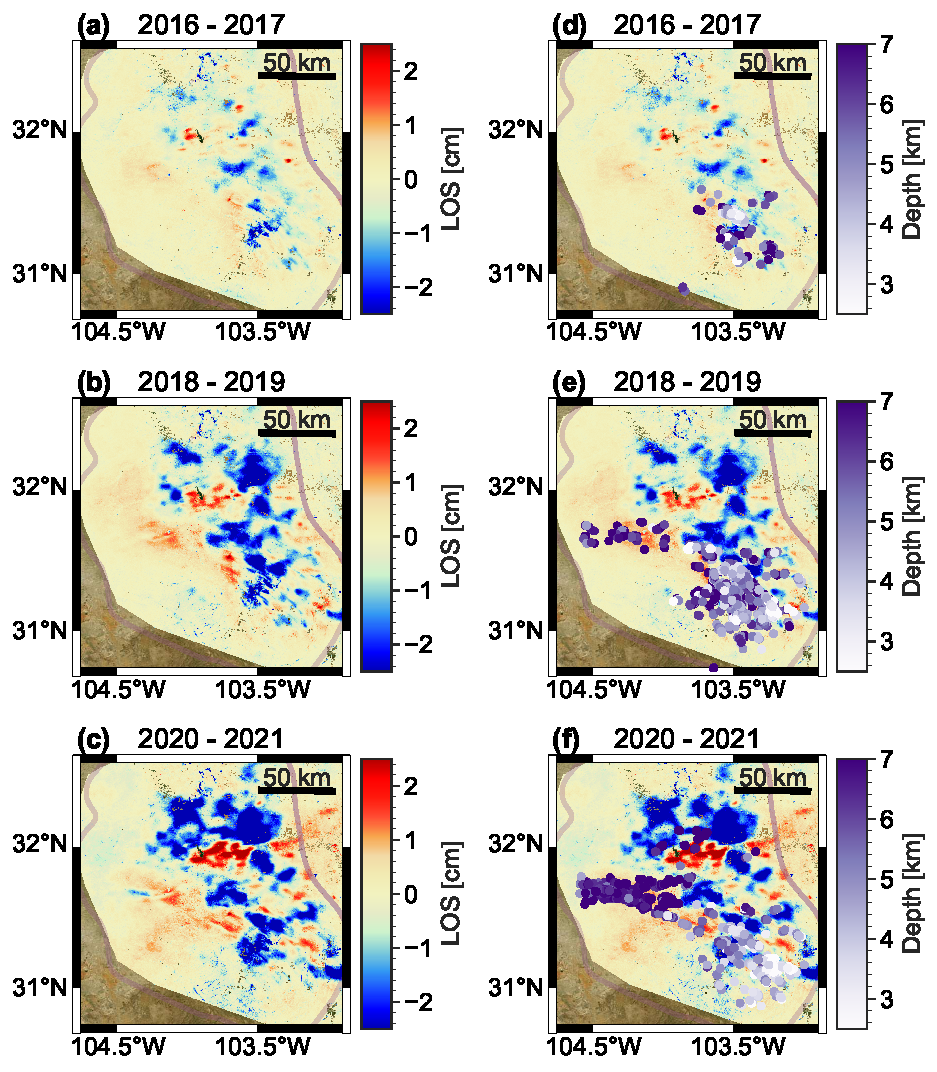
\includegraphics[height=0.85\textheight]{figures/chapter5-lowess/figure-results-eqs.pdf}
	\caption[Earthquakes during two year intervals]{
		Vertical surface deformation for two-year intervals during 2016-2017 (top row), 2018-2019 (middle), and 2020-2021 (bottom). On the left (panel a,b,c) shows the InSAR vertical surface deformation.
		Panels (d,e,f) show the same surface deformation as (a,b,c) with the TexNet earthquakes during the respective time period.
	}
	\label{fig:ch5-discuss-eqs}
\end{figure}


%pressure increases in the three DMG formations \citep{Ge2022RecentWaterDisposal}.



\begin{figure}
	\centering
	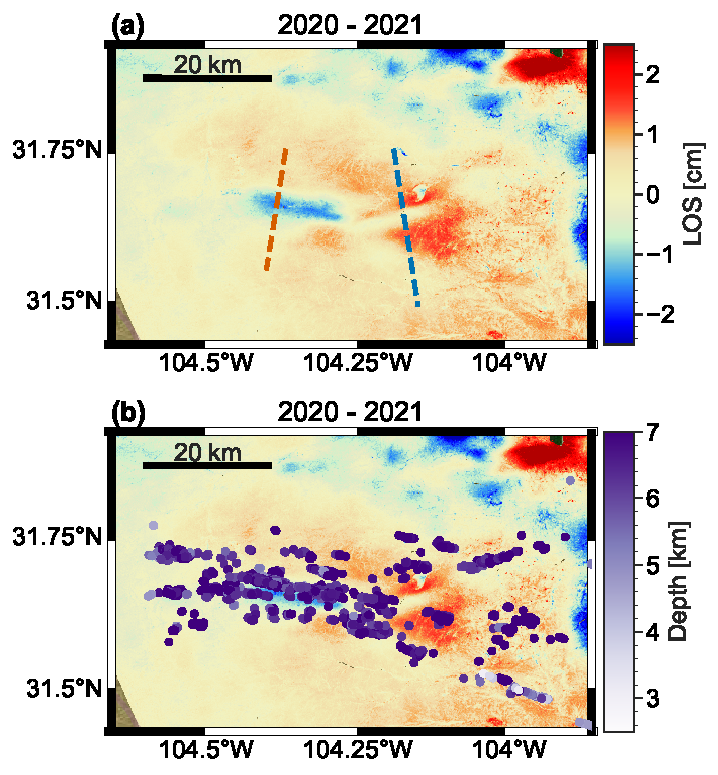
\includegraphics[width=.98\textwidth]{figures/chapter5-lowess/figure-cmez-zoom-transect.pdf}
	\caption[Culberson-Mentone Earthquake Zone earthquakes during 2020 - 2021]{
		(a) Vertical surface deformation for two-year interval during 2020-2021. 
		TexNet earthquakes (black dots) during 2020 - 2021 in the Culberson-Mentone Earthquake Zone (CMEZ) region. Hypocenters shown were relocated using GrowClust \citep{Trugman2017GrowclustHierarchicalClustering}, availabe through \url{https://hirescatalog.texnet.beg.utexas.edu/}.
		Vertical surface deformation along transects (dashed lines) from panel (a) for two-year intervals of 2016-2017 (blue line), 2018-2019 (orange), and 2020-2021 (green). Both transects run from north to south as distance increases.
	}
	\label{fig:ch5-discuss-cmez-transects}
\end{figure}




%Figure: Earthquakes through Jan 2019. Then EQs after (showing CMEZ)

% Figure? Transect of the fault over time, lots of lines


%1. Limitations of stacking to long time series
%2. Robust Time Series Methods
   %1. Regularization (Supplement from GRL)
   %2. LOWESS smoothing
%3. Synthetic Example
%4. 7-year Time Series for the Permian Basin
%1. Comparison to GPS
%2. Anthropogenic Caused Deformation Patterns


%Problems with pixelwise uq
%- Image of blob, with 8 mm cutoff, question which part you trust and not
%- Leads into feature-wise uq




